\documentclass[10pt]{article}
\usepackage[margin=1in]{geometry}
\usepackage{graphicx,booktabs,amsmath,amssymb,xcolor,caption,enumitem,multirow,placeins}
\usepackage[hidelinks,colorlinks=true,linkcolor={blue!55!black},citecolor={blue!55!black},urlcolor={blue!55!black}]{hyperref}
\captionsetup{font=small,labelfont=bf,width=.94\textwidth}
\setlist{itemsep=2pt,topsep=3pt}
% keep figures with their text rather than on near-empty pages
\renewcommand{\topfraction}{0.92}
\renewcommand{\bottomfraction}{0.80}
\renewcommand{\textfraction}{0.06}
\renewcommand{\floatpagefraction}{0.70}
\setcounter{topnumber}{3}
\setcounter{bottomnumber}{2}
\setcounter{totalnumber}{5}
\newcommand{\seq}{\textsc{seq}}
\newcommand{\pl}{\textsc{par}}
\newcommand{\hr}[1]{\texttt{#1}}
\graphicspath{{figs/}}
% long 	exttt tokens cannot hyphenate; let TeX stretch interword space
% rather than run past the margin
\emergencystretch=3.2em
\hbadness=3000

\title{\textbf{BeliefLens: Belief Dynamics in Real LLM Forecasting Systems}\\[3pt]
\Large Four production harnesses, one date-gated sandbox}
\author{BeliefLens Project\\\small Deep Digital Intelligence \; · \;
\url{https://github.com/DDI-droid/belieflens}}
\date{September 11, 2026 \; · \; Experiment~1, v2}

\begin{document}
\maketitle

\begin{abstract}
LLM forecasters are \emph{judgmental} forecasters: behind every stated probability is something
that behaves like a belief, and behind every revision an update rule. This report measures both,
for four \textbf{real forecasting systems} rather than prompt-level imitations of them. We take the
orchestration code of Analytica, of the FutureSim benchmark's reference agent, and of the BLF
sequential-Bayesian forecaster, trim each only where the sandbox requires, and run them alongside
ReAct---which needs no adaptation, being a prompt pattern over a tool loop---inside a date-gated
replay environment built on 339{,}801 news articles. Six binary questions, drawn as three matched
pairs from the FutureSim benchmark's own question set, are forecast under two protocols:
\textbf{sequential} (a trajectory of dates, the system's own state carried forward, $k{=}5$
rollouts) and \textbf{parallel} (a fresh one-shot run per date with no history, $k{=}5$ rollouts),
so that every belief is a distribution and the effect of carrying history is isolated by
construction. A sixth date, placed two days \emph{after} each question resolves, serves as an
\textbf{outcome probe}: by then the corpus contains the answer, so it measures whether a system
moves to the truth when the truth is available.
Findings. Update gain---how far a carried belief moves when the evidence moves---separates the
four systems by a factor of nine, from $0.08$ to $0.74$. Analytica's architecture makes it the
most rigid tracker and simultaneously the most internally coherent, producing near-additive
paired beliefs without ever seeing both halves of a pair. The outcome probe reveals an inversion
invisible to any trajectory metric: the system that tracks evidence best under uncertainty
(\hr{blf-full}, gain $0.74$) is the worst at absorbing a decided outcome, landing $0.46$ from the
truth with the answer in its own search results, while the system that searches least
(\hr{futuresim-full}, $1.3$ searches per forecast) resolves five of six questions exactly. In both
cases the behaviour is traceable to a specific line of architecture rather than to model
capability. All 1{,}432 logged searches in the audit replay with zero articles past the date gate.
\end{abstract}

%=========================================================================
\section{Introduction}
Benchmarks score LLM forecasting agents on outcomes, and observe behaviours---anchoring to initial
forecasts, ``self-conditioning'' on past rationales---that are claims about \emph{belief dynamics}.
But a score cannot say where a pathology lives: in what the agent \emph{believes}, in how it
\emph{updates}, or in how it \emph{gathers evidence}. Those are three different failures with three
different fixes, and one number per condition cannot separate them.

This report separates them, for systems as they are actually built. That last clause is the
methodological commitment. It is easy, and common, to study ``a ReAct-style agent'' or ``an
Analytica-style decomposition'' by writing a prompt that describes the reasoning shape and running
it on a shared loop. We did exactly that in an earlier iteration of this project, and it produced
results that did not survive contact with the real systems: when a structure is \emph{requested in
a prompt} the model may quietly decline it, and when the same structure is \emph{enforced in
orchestration code} it cannot. Everything reported here runs the orchestration.

\paragraph{Contributions.}
\begin{itemize}
\item \textbf{Four real systems in one sandbox.} Analytica's analyzer/grounder/synthesizer
pipeline with its linear composition computed in code; the FutureSim benchmark's own reference
agent with its session architecture, pandas-backed task state and CRUD memory; the BLF forecaster's
Algorithm~1 with $K$-trial shrunken logit-mean aggregation; and ReAct. Each is trimmed only where
the sandbox requires, and every trim is stated (\S\ref{sec:harness}).
\item \textbf{A protocol that isolates history.} Sequential and parallel arms over an identical
date grid, $k{=}5$ rollouts each, so the effect of carrying state is a measured difference rather
than an inference (\S\ref{sec:protocol}).
\item \textbf{The outcome probe.} A date placed after resolution, when the corpus contains the
answer. It converts ``is this system rigid?'' from a relative question into an absolute one, and
it exposes a tracking/resolving inversion that no trajectory metric can see (\S\ref{sec:probe}).
\item \textbf{Matched question pairs.} Three two-sided contests binarised into both finalists, so
coherence---$P(a)+P(b)$, which must not exceed 1 and should approach it as the field narrows---is
measurable on every group, and the resolved answers are balanced three YES to three NO
(\S\ref{sec:questions}).
\end{itemize}

%=========================================================================
\section{Background: the source systems}\label{sec:bg}
\paragraph{Analytica~\cite{analytica}.} Three agent roles, two algorithms. \textsc{Analyze} expands
a root proposition into a tree of sub-propositions until a leaf budget. \textsc{Synthesize} walks
the tree bottom-up: \emph{Grounder} agents evaluate all leaves \emph{in parallel}, each returning a
soft truth value and a written report, and a \emph{Synthesizer} scores each non-leaf from its
children under a \textbf{linear} rule $p=\beta_0+\sum_j\beta_j p_j$, where the LLM emits the
coefficients and the arithmetic is not the model's job. Their §4.1 also defines \textbf{resynthesis}:
after grounding, a user may edit any node and the system recomputes only the affected branches. Our
continual-forecasting extension is exactly that mechanism driven by a calendar.

\paragraph{FutureSim~\cite{futuresim}.} A chronological, replayable simulation. The environment
enforces two actions, \texttt{submit\_forecast} and \texttt{next\_day}; everything else is the
agent's business. Their reference agent, \texttt{basicAgent}, takes one tool call per turn,
chosen from \texttt{query\_df}, \texttt{search\_news}, four memory CRUD tools,
\texttt{submit\_forecasts} and \texttt{next\_day}. It inspects the question table by writing
Python in a sandbox, and has its
context cleared between sessions so that structured memory and past predictions are all that
survive. Two of their findings motivate this work: agents started from a poor initial forecast set
fail to adapt away from it, and the same agent asked each question \emph{directly} one day before
resolution outperforms itself walking the same information forward day by day.

\paragraph{BLF~\cite{blf}.} An agentic system for \emph{binary} question forecasting. Its belief is
a JSON object---probability, confidence, evidence for and against, open uncertainties---and each
step of its loop returns \emph{both} the next action and the updated belief in one generation.
$T_{\max}{=}10$; submitted probabilities clamp to $[0.05,0.95]$. Around the loop sit $K{=}5$
independent trials aggregated by a shrunken logit-space mean
$\hat p=\sigma\!\left(\alpha\cdot\frac1K\sum_k\mathrm{logit}(p_k)\right)$ with $\alpha$ falling as
between-trial variance rises, plus hierarchical Platt calibration.

\paragraph{ReAct~\cite{react}} interleaves thinking and acting with no imposed structure. Unlike the
other three it \emph{is} a prompt pattern over a tool loop, so there is nothing to re-implement: the
harness here is its source system, exposed one date at a time.

\paragraph{Agent-BRACE~\cite{agentbrace}} supplies the framing question---is an externalised belief
structure the agent's \emph{working} belief, or a report it writes alongside one?---but is a
training method, not an installable harness, so it is not run.

%=========================================================================
\section{Infrastructure}\label{sec:infra}
\subsection{Corpus and date gate}
Articles are the FutureSim corpus (HuggingFace \texttt{shash42/forecast-news}; CCNews-derived,
deduplicated, dated), sliced to the simulation window: 2025-12-01--2026-03-31, indexed to SQLite
FTS5 (BM25), 339{,}801 rows. At simulation date $D$ the search tool returns only articles with
$\text{date}\le D$; \textbf{the constraint is in the SQL, not in the prompt}. The audit re-executes
every logged search against its own turn's date; zero returned articles postdate the gate.

We do not use FutureSim's prebuilt hybrid index. Retrieval here is BM25, weaker than theirs, but
byte-identical across all four harnesses---a constant of the experiment rather than a confound in
it.

\subsection{Model choice}
All four harnesses run on \texttt{gpt-5-mini} (released 2025-08-07). This is a validity decision,
not a cost decision: the questions resolve January--February 2026, so a later model would
\emph{recall} rather than forecast, and a model that already knows the outcome does not move its
belief---destroying the thing being measured.

\subsection{Questions}\label{sec:questions}
\paragraph{Why binary.} Every measurement here needs the belief to be a single number in $[0,1]$:
update gain is a regression slope of $\Delta p$ on $\Delta p$, the anchor gap is a difference of two
probabilities, placement is a percentile within a set of draws. FutureSim's native format is a
distribution over outcomes the agent invents for itself, whose support changes between dates; no
scalar trajectory exists in that world. Two of the three source systems are binary-native---BLF
states it outright, Agent-BRACE attaches a probability to a claim---so the choice is faithful to
them and unfaithful to FutureSim's task format, and we say so. The consequence is that our numbers
are not comparable to FutureSim's benchmark scores.

\paragraph{The groups.} Each group is one free-form question from the FutureSim benchmark split
(\texttt{aljazeera2026Q1}, 330 questions) converted into \emph{two} binary questions, one per
finalist of a two-sided contest. The runner-up in each is read off the source article, not
supplied from memory.

\begin{table}[htbp]\centering\small
\begin{tabular}{@{}llp{7.4cm}c@{}}
\toprule
group & question id & binary question, verbatim as the harness sees it & resolves \\
\midrule
\multirow{2}{*}{hockey} & \hr{hockey\_usa} & Will the United States win the men's ice hockey gold
medal at the Milano Cortina 2026 Winter Olympics? & \textbf{YES} \\[2pt]
 & \hr{hockey\_can} & Will Canada win the men's ice hockey gold medal at the Milano Cortina 2026
Winter Olympics? & NO \\
\midrule
\multirow{2}{*}{ausopen} & \hr{ausopen\_alcaraz} & Will Carlos Alcaraz win the 2026 Australian
Open men's singles title? & \textbf{YES} \\[2pt]
 & \hr{ausopen\_djokovic} & Will Novak Djokovic win the 2026 Australian Open men's singles
title? & NO \\
\midrule
\multirow{2}{*}{superbowl} & \hr{superbowl\_sea} & Will the Seattle Seahawks win Super Bowl
LX? & \textbf{YES} \\[2pt]
 & \hr{superbowl\_ne} & Will the New England Patriots win Super Bowl LX? & NO \\
\bottomrule
\end{tabular}
\caption{The six questions, three resolving YES and three NO. Each group binarises one
free-form question from the benchmark split---\emph{``Which country will win the men's ice hockey
gold medal\ldots?''}, \emph{``Who will win the 2026 Australian Open men's singles title?''},
\emph{``Which NFL team will win Super Bowl LX?''}---into its two finalists. Each question is put
to the harness on its own, fully self-contained, with background text that names the event and
date but neither finalist, so a harness forecasting one half of a pair has no way to know the
other half exists. That is what makes coherence an observation about the system rather than an
artefact of the setup.}
\label{tab:questions}
\end{table}

\paragraph{The date grid.} Six dates per question, as offsets from the resolution date $R$. The
forecasting trajectory is $D_1$ at $R{-}39$, then $R{-}25$, $R{-}14$, $R{-}7$ and $D_5$ at
$R{-}2$, accelerating toward the event; then $D_6$ at $R{+}2$, the \textbf{outcome probe}.

\begin{figure}[htbp]\centering

\includegraphics[width=.96\textwidth]{fig_timeline.pdf}
\caption{\textbf{The date grid.} Five trajectory dates per question, then a probe date two days
after resolution. $D_6$ is a diagnostic, not part of the trajectory: by then the corpus contains
the result, so every dynamics metric in this report is computed on $D_1..D_5$ only. Mixing a
post-outcome date into a belief-dynamics slope would corrupt it.}
\label{fig:timeline}
\end{figure}

%=========================================================================
\section{The four harnesses}\label{sec:harness}
Each system runs its own orchestration. The LLM is confined to the roles its paper gives it, and
the composition, control flow and state are executed in code. What follows is what each system is,
and precisely what we changed.

\subsection{\hr{analytica-full}}
An \emph{analyzer} agent decomposes the question into soft sub-propositions (leaf budget 8, up to
three expansion rounds on the first date); parallel per-leaf \emph{grounder} agents each generate
search queries, read gated articles and conclude a leaf probability with a written report in a
separate second call; a \emph{synthesizer} agent assigns weights; and the composition
$p=\mathrm{clamp}(\beta_0+\sum_i\beta_i p_i)$ is computed recursively \emph{in Python}. The model
never states the final probability.

The paper is single-shot, so continual forecasting needs an extension---and the extension is the
paper's own resynthesis mechanism driven by a calendar. The tree is carried as state; each date
runs an analyzer \textbf{edit pass}; every leaf is re-grounded but \textbf{delta-grounded}, its
search window restricted to the period since \emph{that leaf} last looked and its own previous
value shown to it; synthesizer weights are re-elicited \textbf{only} where a node's children
changed.

\begin{figure}[htbp]\centering

\includegraphics[width=.93\textwidth]{fig_arch_analytica.pdf}
\caption{\textbf{Analytica, published versus as run.} Highlighted boxes are the whole
continual-forecasting delta; the composition arithmetic is unchanged.}
\label{fig:arch-analytica}
\end{figure}

\subsection{\hr{blf-full}}
Algorithm~1 verbatim in structure: an explicit JSON belief state; each step one generation
returning both an action and the updated belief; $T_{\max}{=}10$; the submitted probability clamped
to $[0.05,0.95]$; $K{=}5$ trials per date aggregated by the paper's shrunken logit-space mean with
$\alpha=1/(1+\mathrm{Var}(\mathrm{logit}(p_k)))$---our instantiation of their variance-dependent
$\alpha$, whose functional form they do not pin down. The belief state of the median-probability
trial carries across dates in \seq{} and is rebuilt from scratch in \pl. Their \texttt{LeakFilter},
a second-pass LLM filter on search results, is replaced by our SQL date gate, which is strictly
stronger. Platt calibration is omitted: it requires resolved training questions, and the window
contains none.

\begin{figure}[htbp]\centering

\includegraphics[width=.93\textwidth]{fig_arch_blf.pdf}
\caption{\textbf{BLF, published versus as run.} Note that $K$ is \emph{internal}: the five trials
collapse to one number, which is that date's forecast. It is not our rollout count.}
\label{fig:arch-blf}
\end{figure}

\subsection{\hr{futuresim-full}}
The FutureSim benchmark's own reference agent. Context is cleared between dates, so structured
memory and past predictions are all that survive; one tool call per turn from their action set;
\texttt{query\_df} is a real pandas sandbox over the question table with \texttt{pd} in scope;
memory is four CRUD tools plus a separate end-of-session memory-revision phase;
\texttt{submit\_forecasts} takes a distribution over outcomes, from which we read $P(\text{Yes})$.

Two changes. We drive the calendar rather than letting the agent advance it, so that all four
harnesses share one date grid and remain comparable. And the agent must submit on every date: their
system permits ending a session without submitting, leaving the standing forecast in place, and
disabling that is the single largest liberty this report takes with a source system.

\begin{figure}[htbp]\centering
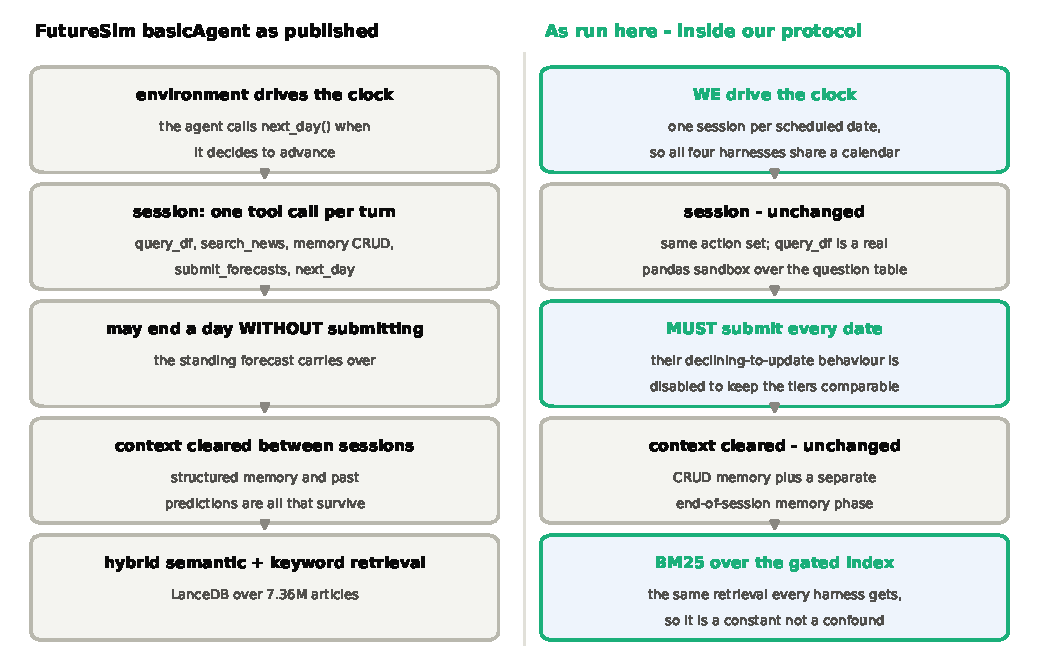
\includegraphics[width=.90\textwidth]{fig_arch_futuresim.pdf}
\caption{\textbf{FutureSim's reference agent, published versus as run.}}
\label{fig:arch-futuresim}
\end{figure}

\subsection{\hr{react}}
A think/search/read loop with no imposed structure, at most six search rounds, then a forced
answer. ReAct is a prompt pattern over a tool loop, so this harness \emph{is} its source system;
the only adaptation is exposing it one date at a time.

\FloatBarrier
%=========================================================================
\section{Protocols and metrics}\label{sec:protocol}
\textbf{Sequential (\seq)}: the five trajectory dates in order; each date the harness sees its own
previous forecasts and whatever state its architecture carries (Analytica's tree, BLF's belief JSON,
FutureSim's memory); $k{=}5$ independent rollouts of the whole trajectory.
\textbf{Parallel (\pl)}: for each date, a fresh run given all information up to that date and
\emph{no} history; $k{=}5$ rollouts per date. The parallel arm is what the evidence alone supports;
the difference between the arms is what carrying history does.

\begin{description}[leftmargin=1.6cm,style=nextline,itemsep=1pt]
\item[anchor gap] $\seq_t-\overline{\pl}_t$, signed, for $t\ge2$. What carrying history does
relative to evidence alone.
\item[lag advantage] $|\seq_t-\overline{\pl}_t|-|\seq_t-\overline{\pl}_{t-1}|$. Positive means the
sequence tracks \emph{yesterday's} evidence-conditioned belief better than today's.
\item[update gain] OLS slope of $\Delta\seq_t$ on $\Delta\overline{\pl}_t$. $1$ means the carried
belief moves exactly as far as the evidence moves; $<1$ is conservatism; $<0$ moves against it.
\item[placement (PIT)] Percentile of each sequential forecast within that date's parallel draws;
$50$ is unbiased.
\item[stabilisation] $\mathrm{sd}(\seq)/\mathrm{sd}(\pl)$ per date. Below 1 means carrying history
reduces variance across rollouts.
\item[coherence] $P(a)+P(b)$ within a matched group. Must not exceed 1; should approach it as the
field narrows to the two candidates.
\item[total movement] $|\Delta|_\text{tot}$, the summed absolute day-to-day change of a rollout.
\item[Brier] The plain quadratic score $\frac1n\sum_i(p_i-y_i)^2$ with $y_i\in\{0,1\}$---not a
skill score. $0$ is perfect and \textbf{0.25} is the constant-$\tfrac12$ forecaster.
\end{description}

\noindent Every metric above is computed on $D_1..D_5$. The probe date is reported separately in
\S\ref{sec:probe}.

%=========================================================================
\section{Results}\label{sec:results}

\begin{table}[htbp]\centering\small
\begin{tabular}{@{}lrrrrrrr@{}}
\toprule
harness & $|\Delta|_\text{tot}$ & gap & $|$gap$|$ & \textbf{gain} & PIT$_{\mathrm{med}}$ &
lag adv. & searches \seq/\pl \\
\midrule
\hr{analytica-full} & 0.243 & $-0.006$ & 0.128 & \textbf{0.08} & 40 & $+0.016$ & 6.8 / 6.6 \\
\hr{blf-full} & 0.184 & $-0.031$ & \textbf{0.047} & \textbf{0.74} & \textbf{0} & $-0.012$ &
\textbf{22.8 / 25.2} \\
\hr{futuresim-full} & \textbf{0.274} & $+0.029$ & 0.079 & 0.45 & 60 & $-0.023$ &
\textbf{1.3 / 1.2} \\
\hr{react} & 0.240 & $-0.012$ & 0.067 & 0.45 & 40 & $-0.019$ & 2.6 / 2.6 \\
\bottomrule
\end{tabular}
\caption{\textbf{Headline metrics}, $k{=}5$ in both arms, pooled over six questions and five
trajectory dates ($n{=}1{,}200$ forecasts). Bold marks the extreme of each column.}
\label{tab:headline}
\end{table}

\subsection{Update gain separates the systems by a factor of nine}
The single most discriminating number in the table is update gain, and it ranges from $0.08$ to
$0.74$. \hr{analytica-full} moves its carried belief eight points for every hundred points the
evidence moves. \hr{blf-full} moves seventy-four.

\begin{figure}[htbp]\centering

\includegraphics[width=.97\textwidth]{fig_gain.pdf}
\caption{\textbf{Update gain.} Each dot is one date-step: $x$ is the movement of the fresh-eyes
mean, $y$ the movement of a sequential rollout; the dashed diagonal is $y{=}x$, perfect tracking.}
\label{fig:gain}
\end{figure}

Analytica's rigidity is traceable to three specific lines of its architecture, none of which is an
instruction a model may decline. A leaf that searches only news \emph{since it last looked} cannot
react to standing evidence it has already discounted. A leaf handed its own prior value is anchored
by design. And a parent whose children did not change reuses yesterday's weights outright. The
belief is structurally prevented from responding to evidence that does not survive the edit pass.

\paragraph{A result that did not replicate.} An earlier iteration of this experiment, run on two
questions with $K{=}3$, measured \hr{blf-full}'s update gain at $-0.17$ and reported it as evidence
that the system moved \emph{against} the evidence---flagged at the time as weakly identified,
because its fresh-eyes mean rarely moved more than $\pm0.06$ and the slope was fitted over a very
narrow range. At six questions and $K{=}5$ the same measurement gives $+0.74$. The earlier number
was not merely imprecise, it had the wrong sign. We report this prominently because it is the
clearest available evidence that two questions cannot support a claim of this kind, and because
the failure mode---a slope confidently estimated over a degenerate $x$-range---is not specific to
this project.

\begin{figure}[htbp]\centering
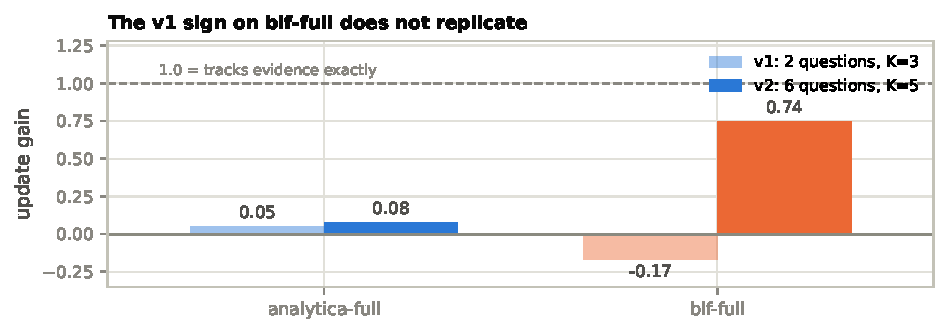
\includegraphics[width=.72\textwidth]{fig_replication.pdf}
\caption{\textbf{Non-replication.} The same metric, the same harness, the same code path;
two questions at $K{=}3$ against six questions at $K{=}5$.}
\label{fig:replication}
\end{figure}

\subsection{Anchoring, placement and stabilisation}
The signed anchor gaps are small for every system ($|{\cdot}|\le0.031$), so none of them holds a
systematically higher or lower belief than fresh eyes would. What differs is dispersion:
\hr{analytica-full}'s \emph{absolute} gap is $0.128$, nearly three times \hr{blf-full}'s $0.047$,
so its carried belief wanders far from the evidence-conditioned one in both directions without a
net bias.

\begin{figure}[htbp]\centering

\includegraphics[width=.9\textwidth]{fig_anchor.pdf}
\caption{\textbf{Anchoring summary.} Left: signed anchor gap. Right: lag advantage; only
\hr{analytica-full} is positive, and only slightly.}
\label{fig:anchor}
\end{figure}

\hr{blf-full}'s placement median of $\mathbf{0}$ deserves care. It means its sequential forecast
sits at or below \emph{every} parallel draw, essentially always. That sounds extreme until one
notices its $K{=}5$ aggregation makes the parallel draws exceptionally tight---so a signed gap of
only $-0.031$ is enough to fall below all five. The placement statistic is measuring the
aggregator's variance reduction as much as the belief's bias, and should not be read as strong
anchoring.

\begin{figure}[htbp]\centering

\includegraphics[width=.97\textwidth]{fig_stab_pit.pdf}
\caption{\textbf{Left:} stabilisation ratio. \hr{react} is the only system consistently below 1:
carrying history genuinely reduces its cross-rollout variance. \hr{blf-full} sits above 1
throughout, peaking at $2.09$---carrying the belief state makes its rollouts \emph{diverge},
consistent with the carried JSON acting as a strong per-rollout prior that each trajectory then
drags along its own path. \textbf{Right:} placement.}
\label{fig:stab}
\end{figure}

\subsection{Coherence comes from architecture}
\hr{analytica-full} produces near-additive paired beliefs on the hockey group---$1.00$, $0.98$,
$1.01$, $1.02$, $0.99$ across the five dates---\emph{without ever seeing the two questions
together}. Decomposition into sub-propositions plus linear synthesis yields consistency as a side
effect of the architecture. No other system comes close on that group; \hr{react} sits at $0.67$
and \hr{blf-full} at $0.74$.

\begin{figure}[htbp]\centering
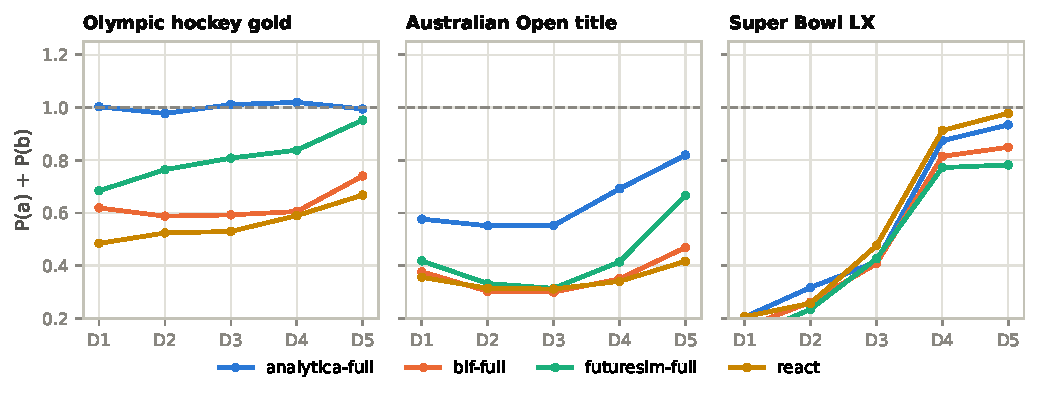
\includegraphics[width=.97\textwidth]{fig_coherence.pdf}
\caption{\textbf{Coherence per group}, $P(a)+P(b)$ against the target of 1. The Super Bowl group
shows every system converging late, as the playoff field narrows to two teams---the sum climbs from
about $0.2$ at $D_1$ to $0.78$--$0.98$ at $D_5$. That is the metric behaving correctly: before the
finalists are known the sum \emph{should} be well below 1.}
\label{fig:coherence}
\end{figure}

\subsection{Accuracy}
All four systems improve monotonically across the window, from a pooled Brier around $0.38$--$0.40$
at $D_1$ to $0.24$--$0.32$ at $D_5$. \hr{blf-full} finishes at $\mathbf{0.240}$, below the
constant-$\tfrac12$ baseline of $0.25$; the others do not clear it.

\begin{figure}[htbp]\centering
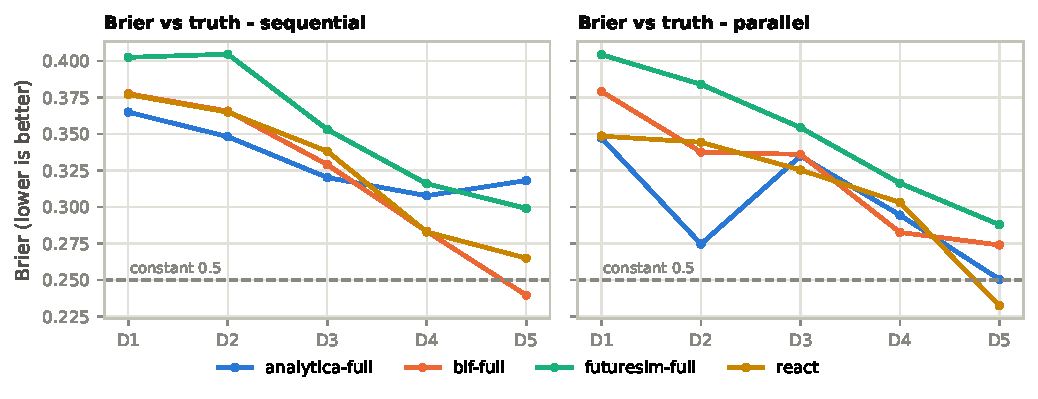
\includegraphics[width=.97\textwidth]{fig_brier.pdf}
\caption{\textbf{Brier against the resolved outcomes}, pooled over the six questions.}
\label{fig:brier}
\end{figure}

\subsection{Search effort varies by a factor of eighteen}
\begin{figure}[htbp]\centering

\includegraphics[width=.9\textwidth]{fig_search.pdf}
\caption{\textbf{Search effort.} \hr{blf-full} issues $22.8$ searches per forecast---five trials
times roughly five queries each---while \hr{futuresim-full} issues $1.3$.}
\label{fig:search}
\end{figure}

\noindent This is where the systems differ most starkly, and the naive reading---that more search
means better forecasting---is wrong in both directions, as the next section shows.

\FloatBarrier
%=========================================================================
\section{The outcome probe}\label{sec:probe}
At $D_6 = R{+}2$ the corpus contains the result. A system that cannot reach the truth here is not
failing at forecasting; it is failing at reading. This turns rigidity from a relative measurement
into an absolute one.

\begin{table}[htbp]\centering\small
\begin{tabular}{@{}lrrr@{}}
\toprule
harness & mean move toward truth & mean $|$forecast $-$ truth$|$ & direction correct \\
\midrule
\hr{futuresim-full} & $\mathbf{+0.498}$ & $\mathbf{0.025}$ & 6/6 \\
\hr{react} & $+0.329$ & $0.134$ & 6/6 \\
\hr{analytica-full} & $+0.252$ & $0.280$ & 6/6 \\
\hr{blf-full} & $\mathbf{+0.014}$ & $\mathbf{0.462}$ & \textbf{3/6} \\
\bottomrule
\end{tabular}
\caption{\textbf{Outcome probe.} \hr{futuresim-full} lands on the truth \emph{exactly}---0.000 or
1.000---on five of the six questions, and at $0.85$ on the sixth. \hr{blf-full} barely moves at
all.}
\label{tab:probe}
\end{table}

\begin{figure}[htbp]\centering

\includegraphics[width=.97\textwidth]{fig_probe.pdf}
\caption{\textbf{Left:} each arrow runs from a system's mean belief at $D_5$ to its mean belief at
$D_6$; the star is the truth. \textbf{Right:} residual error once the answer is public.}
\label{fig:probe}
\end{figure}

\paragraph{The inversion.} \hr{blf-full} has the best update gain of any system measured here
($0.74$) and the worst outcome-probe error ($0.462$, correct direction on only three of six
questions). It is simultaneously the best tracker of uncertain evidence and the worst absorber of
decided fact. The mechanism is not mysterious: its forecast is a shrunken logit-space mean over
five trials, clamped to $[0.05,0.95]$. The clamp alone caps its error at $0.05$ from either
extreme, and the variance shrinkage pulls hardest toward the prior exactly when trials disagree.
The machinery that makes it responsive under uncertainty is the same machinery that prevents it
from committing under certainty.

\paragraph{The other direction.} \hr{futuresim-full} issues $1.3$ searches per forecast, by far the
fewest, and resolves five of six questions exactly. Its low search count is not laziness. When the
signal is decisive one search suffices; the cost is paid earlier in the window, where it has the
weakest Brier of the four at $D_1$--$D_2$. Search volume is a poor proxy for evidence use in either
direction.

\FloatBarrier
%=========================================================================
\section{Synthesis}
Three claims survive the six questions.

\textbf{Rigidity is architectural, and locatable.} The nine-fold spread in update gain is not a
spread in model capability---every system runs the same model on the same corpus behind the same
date gate. Analytica's delta-grounding, weight reuse and per-leaf anchoring produce a gain of
$0.08$; BLF's flat belief with full re-search produces $0.74$. Pointing at the mechanism is
possible because the mechanism is code.

\textbf{Tracking and resolving are different capabilities.} No trajectory metric distinguishes a
system that is appropriately uncertain from one that is structurally incapable of confidence. The
probe does, and it ranks the systems almost in reverse.

\textbf{Consistency can be a side effect of structure.} Analytica's paired beliefs sum to
approximately 1 on the hockey group with no mechanism that could have told it a pair existed. If
coherence is wanted, it appears to be obtainable by construction rather than by instruction.

%=========================================================================
\section{Reproducibility and the data package}\label{sec:data}
Everything below ships in \texttt{results/exp1\_v2/}.

\begin{table}[htbp]\centering\small
\begin{tabular}{@{}llr@{}}
\toprule
file & contents & size \\
\midrule
\texttt{e1\_runs.jsonl} & 120 sequential chains $\times$ 6 dates, with full traces & 5.2 MB \\
\texttt{e1\_independent.jsonl} & 720 parallel singles, with full traces & 5.4 MB \\
\texttt{metrics\_v2.json} & every metric in this report & 85 KB \\
\texttt{usage.json} & call and token ledger & --- \\
\bottomrule
\end{tabular}
\caption{Collected data. 713 of 720 sequential turns and 718 of 720 parallel singles carry a
complete trace; the gaps are exactly the rate-limited forecasts of \S\ref{sec:limits}.}
\label{tab:data}
\end{table}

Traces are per-harness and preserve each system's internal state, which is what makes this dataset
reusable rather than merely a table of probabilities:

\begin{itemize}
\item \hr{analytica-full}: the full proposition tree at every date---each node's statement, its
grounder's written report, its soft truth value, the synthesizer's $\beta$ weights and intercept,
and the date it was last grounded---plus the edit list and every search issued.
\item \hr{blf-full}: the per-trial probabilities, the aggregate, the belief JSON (probability,
confidence, evidence for and against, open uncertainties), and every search tagged by trial and
step.
\item \hr{futuresim-full}: the action sequence, the \texttt{query\_df} code the agent wrote and
what it returned, the memory store and every operation applied to it, and its searches.
\item \hr{react}: the reasoning text, the searches, and whether the answer was forced by exhausting
the search budget.
\end{itemize}

\noindent Reproduce with \texttt{run\_real\_e1.py} for the run, \texttt{analyze\_v2.py} for
the metrics and \texttt{figures\_v2.py} for the figures; \texttt{watch\_run.py} monitors a run
in progress. The key is read from \texttt{.env}.

\paragraph{Cost.} 19{,}385 model calls, 35.1M input and 8.2M output tokens recorded, 2h22m at
twelve workers, against a hard 32{,}000-call cap enforced in the call wrapper. The recorded token
figures exclude \hr{react}, which calls through its own client; its calls are counted but its
tokens are not, so the true token total is roughly 10--15\% higher.

%=========================================================================
\section{Limitations}\label{sec:limits}
\begin{enumerate}
\item \textbf{Six questions, three groups.} Better than two, and enough to overturn a two-question
result (\S\ref{sec:results}), but not enough to support fine distinctions. The gain ordering
$0.08 < 0.45 \approx 0.45 < 0.74$ is coarse and we do not read the tie between
\hr{futuresim-full} and \hr{react} as meaningful.
\item \textbf{All three contests are sport.} They share a structure---a narrowing field, a decisive
public result---that political or economic questions do not. The coherence convergence in
particular may be specific to bracket-shaped events.
\item \textbf{$k{=}5$ rollouts} bounds every distributional claim; placement has five-draw
granularity, which is why a median of exactly 0 is possible.
\item \textbf{Draws are ordinary decoding variation.} Current reasoning endpoints reject
temperature control.
\item \textbf{Stated beliefs only.} Everything here is a consistency property of verbalised
probabilities under intervention, not a claim about internal representations.
\item \textbf{Retrieval is BM25}, weaker than FutureSim's hybrid index. Held constant across
harnesses, so comparisons hold, but absolute accuracy is a lower bound for all four.
\item \textbf{\hr{futuresim-full} is forced to submit every date.} Its source system may decline to
update, and that behaviour---which FutureSim's own anchoring finding is partly about---is disabled
here to keep the harnesses comparable. It is the largest liberty this report takes.
\item \textbf{Nine forecasts of 1{,}440 (0.6\%) were lost} to rate-limit errors that outlived five
retries; 1{,}780 retries were absorbed successfully. The losses are scattered and no cell lost more
than one rollout.
\item \textbf{Binarisation changes the task.} Our numbers are not comparable to FutureSim benchmark
scores, and binary questions are easier than the open-ended originals.
\end{enumerate}

%=========================================================================
\section{Conclusion}
Running four forecasting systems as they are actually built, rather than as prompts describing
them, makes their belief dynamics attributable to specific architecture: delta-grounding and weight
reuse produce rigidity, a flat belief with full re-search produces responsiveness, and shrunken
multi-trial aggregation produces an inability to commit when the evidence is decisive. A date
placed after resolution turns the last of these from an inference into a measurement, and reveals
that the best tracker of uncertain evidence is the worst absorber of certain evidence. The
collected traces preserve each system's internal state at every date, so the same run supports
analysis well beyond the metrics reported here.

\begin{thebibliography}{9}\small
\bibitem{analytica} \emph{Analytica: Soft Propositional Reasoning for Robust and Scalable
LLM-Driven Analysis}. arXiv:2604.23072, 2026.
\bibitem{futuresim} \emph{FutureSim: Replaying World Events to Evaluate Adaptive Agents}.
arXiv:2605.15188, 2026.
\bibitem{agentbrace} \emph{Agent-BRACE: Decoupling Beliefs from Actions in Long-Horizon Tasks via
Verbalized State Uncertainty}. arXiv:2605.11436, 2026.
\bibitem{react} \emph{ReAct: Synergizing Reasoning and Acting in Language Models}. ICLR, 2023.
\bibitem{blf} \emph{Agentic Forecasting using Sequential Bayesian Updating of Linguistic Beliefs}.
arXiv:2604.18576, 2026.
\bibitem{brier} \emph{Verification of forecasts expressed in terms of probability}. Monthly Weather
Review, 1950.
\end{thebibliography}

\clearpage
\appendix
\section{Belief trajectories, all four systems}\label{app:flow}
\begin{figure}[htbp]\centering
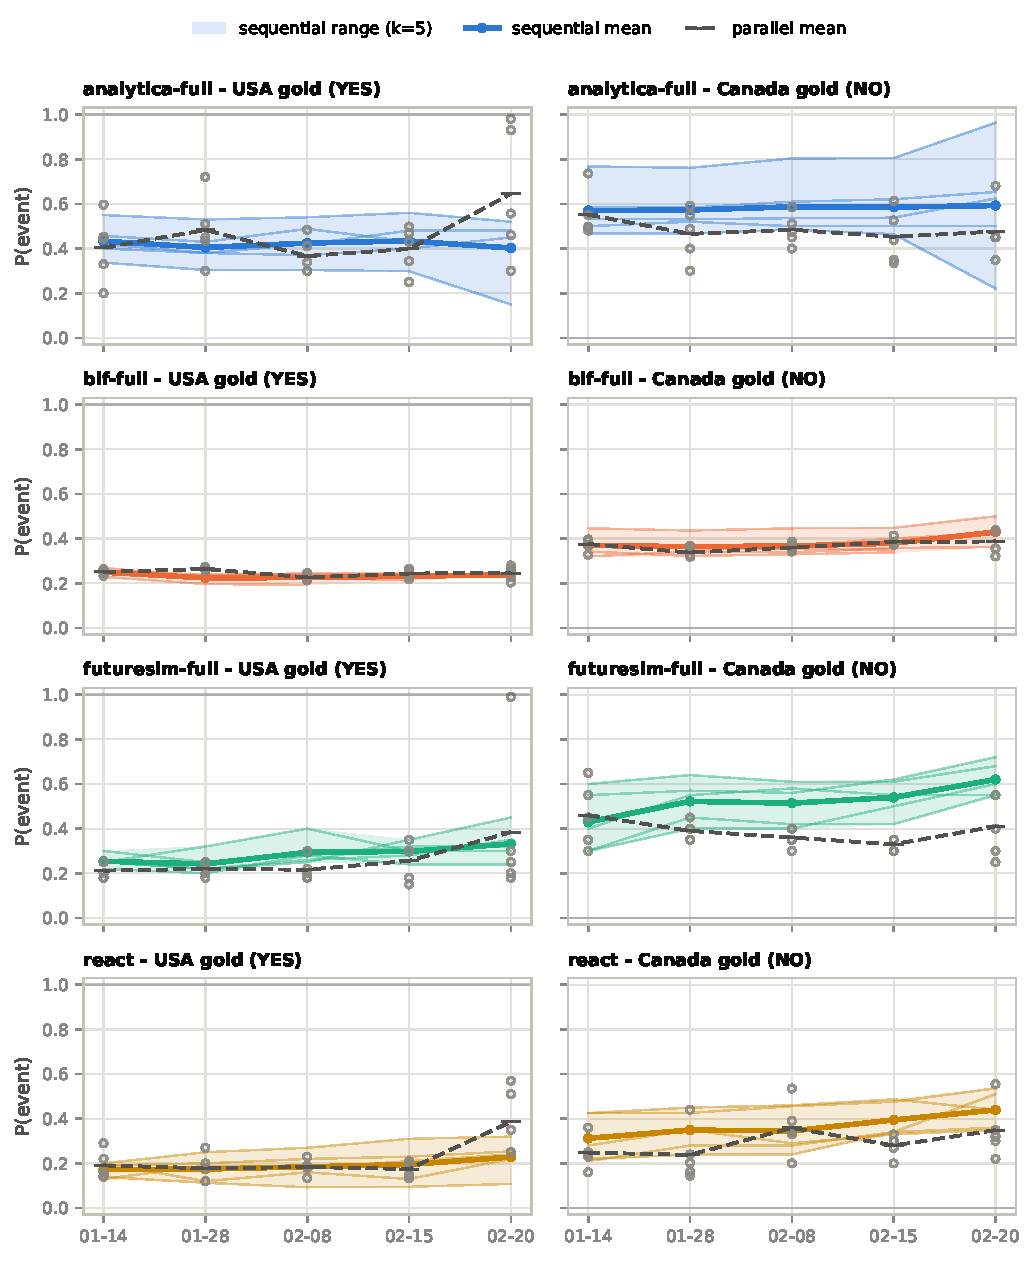
\includegraphics[width=.93\textwidth]{fig_flow_hockey.pdf}
\caption{\textbf{Olympic hockey gold.} Shaded band and bold line: range and mean of the five
sequential rollouts. Open dots and dashed line: the five parallel draws per date and their mean.
Horizontal line: the resolved truth.}
\label{fig:flow-hockey}
\end{figure}

\begin{figure}[htbp]\centering
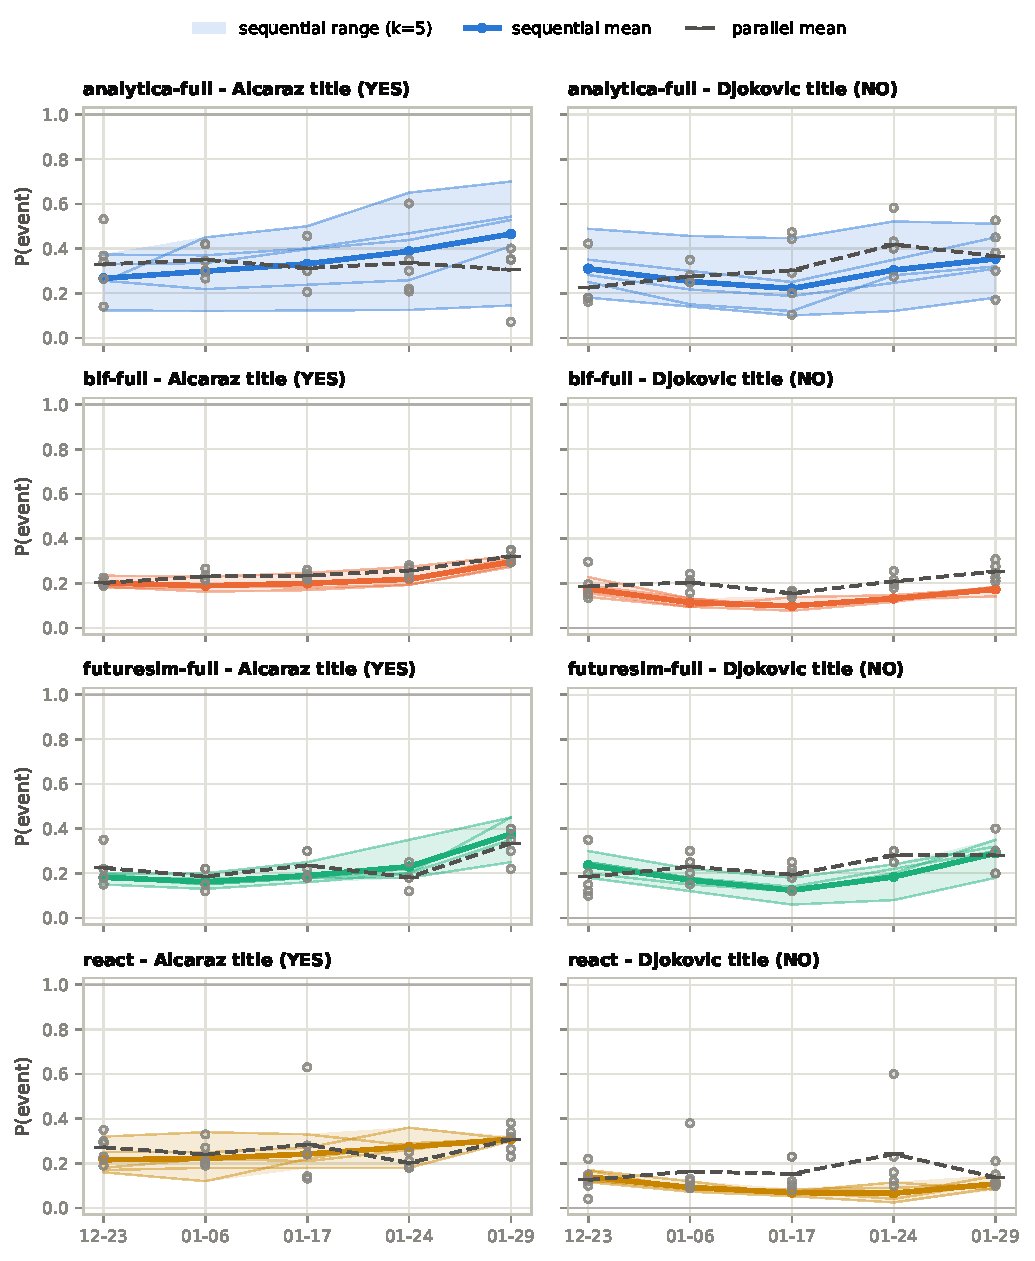
\includegraphics[width=.93\textwidth]{fig_flow_ausopen.pdf}
\caption{\textbf{Australian Open title.}}
\label{fig:flow-ausopen}
\end{figure}

\begin{figure}[htbp]\centering
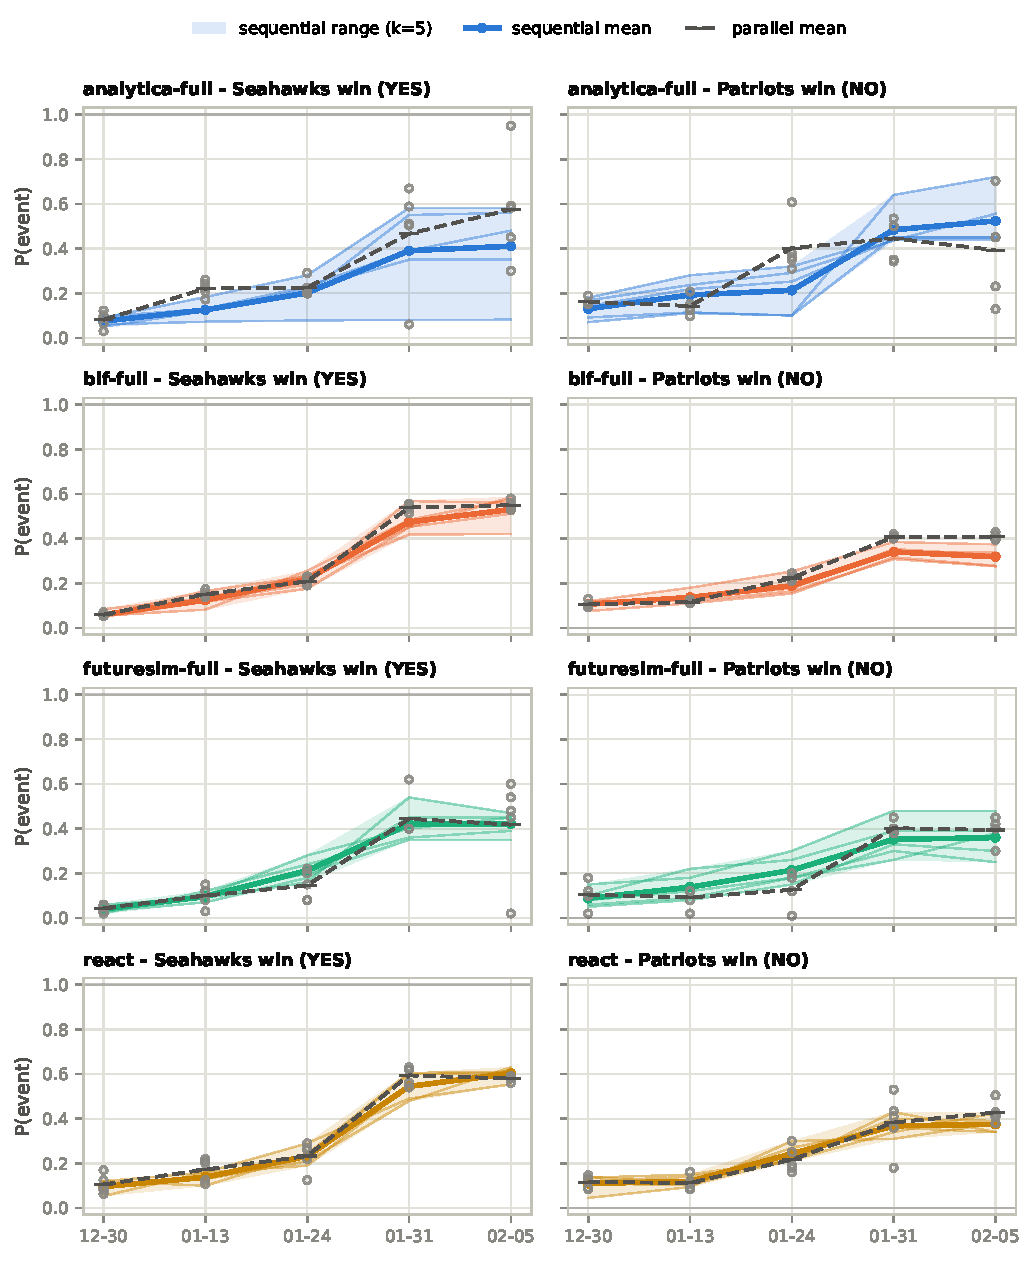
\includegraphics[width=.93\textwidth]{fig_flow_superbowl.pdf}
\caption{\textbf{Super Bowl LX.}}
\label{fig:flow-superbowl}
\end{figure}

\FloatBarrier
\section{Per-question outcome probe}\label{app:probe}
\begin{table}[htbp]\centering\small
\begin{tabular}{@{}llrrr@{}}
\toprule
harness & question & truth & $D_5$ & $D_6$ \\
\midrule
\multirow{6}{*}{\hr{analytica-full}}
 & \hr{hockey\_usa} & 1 & 0.40 & 0.64 \\
 & \hr{hockey\_can} & 0 & 0.59 & 0.46 \\
 & \hr{ausopen\_alcaraz} & 1 & 0.47 & 0.82 \\
 & \hr{ausopen\_djokovic} & 0 & 0.35 & 0.32 \\
 & \hr{superbowl\_sea} & 1 & 0.41 & 0.80 \\
 & \hr{superbowl\_ne} & 0 & 0.52 & 0.17 \\
\midrule
\multirow{6}{*}{\hr{blf-full}}
 & \hr{hockey\_usa} & 1 & 0.24 & 0.25 \\
 & \hr{hockey\_can} & 0 & 0.43 & 0.42 \\
 & \hr{ausopen\_alcaraz} & 1 & 0.30 & 0.45 \\
 & \hr{ausopen\_djokovic} & 0 & 0.17 & 0.30 \\
 & \hr{superbowl\_sea} & 1 & 0.53 & 0.56 \\
 & \hr{superbowl\_ne} & 0 & 0.32 & 0.31 \\
\midrule
\multirow{6}{*}{\hr{futuresim-full}}
 & \hr{hockey\_usa} & 1 & 0.33 & 0.85 \\
 & \hr{hockey\_can} & 0 & 0.62 & \textbf{0.00} \\
 & \hr{ausopen\_alcaraz} & 1 & 0.38 & \textbf{1.00} \\
 & \hr{ausopen\_djokovic} & 0 & 0.29 & \textbf{0.00} \\
 & \hr{superbowl\_sea} & 1 & 0.42 & \textbf{1.00} \\
 & \hr{superbowl\_ne} & 0 & 0.36 & \textbf{0.00} \\
\midrule
\multirow{6}{*}{\hr{react}}
 & \hr{hockey\_usa} & 1 & 0.23 & 0.30 \\
 & \hr{hockey\_can} & 0 & 0.44 & 0.10 \\
 & \hr{ausopen\_alcaraz} & 1 & 0.31 & \textbf{1.00} \\
 & \hr{ausopen\_djokovic} & 0 & 0.11 & \textbf{0.00} \\
 & \hr{superbowl\_sea} & 1 & 0.60 & \textbf{1.00} \\
 & \hr{superbowl\_ne} & 0 & 0.38 & \textbf{0.00} \\
\bottomrule
\end{tabular}
\caption{Mean sequential forecast at the last trajectory date and at the probe. Bold marks an exact
hit. \hr{blf-full} moves by more than $0.05$ on only two of six questions.}
\label{tab:probe-full}
\end{table}

\FloatBarrier
\section{Per-date series}\label{app:series}
\begin{table}[htbp]\centering\small
\begin{tabular}{@{}llrrrrr@{}}
\toprule
harness & series & $D_1$ & $D_2$ & $D_3$ & $D_4$ & $D_5$ \\
\midrule
\multirow{2}{*}{\hr{analytica-full}} & stabilisation & 0.85 & 1.25 & 1.26 & 1.06 & 0.93 \\
 & Brier \seq/\pl & .365/.347 & .348/.275 & .320/.335 & .308/.294 & .318/.250 \\
\midrule
\multirow{2}{*}{\hr{blf-full}} & stabilisation & 1.07 & 1.59 & 2.09 & 1.71 & 1.13 \\
 & Brier \seq/\pl & .378/.379 & .366/.338 & .329/.336 & .283/.283 & .240/.274 \\
\midrule
\multirow{2}{*}{\hr{futuresim-full}} & stabilisation & 0.68 & 1.07 & 1.02 & 1.33 & 0.48 \\
 & Brier \seq/\pl & .403/.404 & .405/.384 & .353/.354 & .316/.316 & .299/.288 \\
\midrule
\multirow{2}{*}{\hr{react}} & stabilisation & 0.90 & 0.67 & 0.58 & 0.76 & 0.59 \\
 & Brier \seq/\pl & .377/.349 & .365/.344 & .338/.325 & .283/.303 & .265/.232 \\
\bottomrule
\end{tabular}
\caption{Indexed by trajectory step rather than calendar date, because the three groups resolve on
different dates. Stabilisation is $\mathrm{sd}(\seq)/\mathrm{sd}(\pl)$.}
\label{tab:series}
\end{table}

\end{document}
